\section{Tradução dirigida pela sintaxe}

\begin{frame}[fragile]{Notação posfixa}

    \begin{block}{Definição de notação posfixa}
    A notação posfixa para uma expressão $E$ é definida da seguinte maneira:

    \begin{enumerate}
        \item Se $E$ for uma variável ou uma constante, então a notação posfixa para $E$ é o próprio $E$

        \item Se $E$ é uma expressão da forma $E_1\ op\ E_2$, onde $op$ é um operador binário, então a forma posfixa para $E$ é $E'_1\ E'_2\ op$, onde $E'_1$ e 
            $E'_2$ são as notações posfixas de $E_1$ e $E_2$, respectivamente

        \item Se $E$ é uma expressão da forma $(E_1)$, então a notação posfixa para $E_1$ será a notação posfixa para $E$
    \end{enumerate}
    \end{block}

\end{frame}

\begin{frame}[fragile]{Definições dirigidas pela sintaxe}

    \begin{itemize}
        \item Uma definição dirigida pela sintaxe usa a gramatica livre de contexto para especificar a estrutura sintática da entrada
       %\pause

        \item Ela associa, a cada símbolo da gramática, um conjunto de atributos e, a cada produção, um conjunto de regras semânticas para computar os valores
            dos atributos associados aos símbolos presentes na produção
       %\pause

        \item A gramática e o conjunto de regras semânticas constiturem a definição dirigida pela sintaxe
       %\pause

        \item Um atributo é dito sintetizado se seu valor depende apenas dos valores dos atributos dos nós filhos de seu nó na árvore gramatical
       %\pause

        \item Os atributos sintetizados podem ser computados por meio de uma travessia por profundidade
    \end{itemize}

\end{frame}

\begin{frame}[fragile]{Definição dirigida pela sintaxe para a tradução de notação infixa para posfixa}

    \begin{center}
    \begin{tabular}{ll}
        \toprule
        \textbf{Produção} & \textbf{Regra semântica} \\
        \midrule
        $expr \to expr_1 + digito$ & $expr.t := expr_1.t\ ||\ digito.t\ ||\ $ \code{cpp}{'+'}\\
        $expr \to expr_1 - digito$ & $expr.t := expr_1.t\ ||\ digito.t\ ||\ $ \code{cpp}{'-'}\\
        $expr \to digito$ & $expr.t := digito.t$ \\
        $digito \to 0$ & $digito.t :=$ \code{cpp}{'0'} \\
        $digito \to 1$ & $digito.t :=$ \code{cpp}{'1'} \\
        $\ldots$ & $\ldots$ \\
        $digito \to 9$ & $digito.t :=$ \code{cpp}{'9'} \\
        \bottomrule
    \end{tabular}
    \end{center}

    \vspace{0.2in}

    A notação $X.t$ indica que $t$ é um atributo de $X$ e $||$ indica concatenação de caracteres.
\end{frame}

\begin{frame}[fragile]{Valores dos atributos nos nós da árvore gramatical da expressão \code{cpp}{1-2+3}}

    \begin{figure}
        \centering

        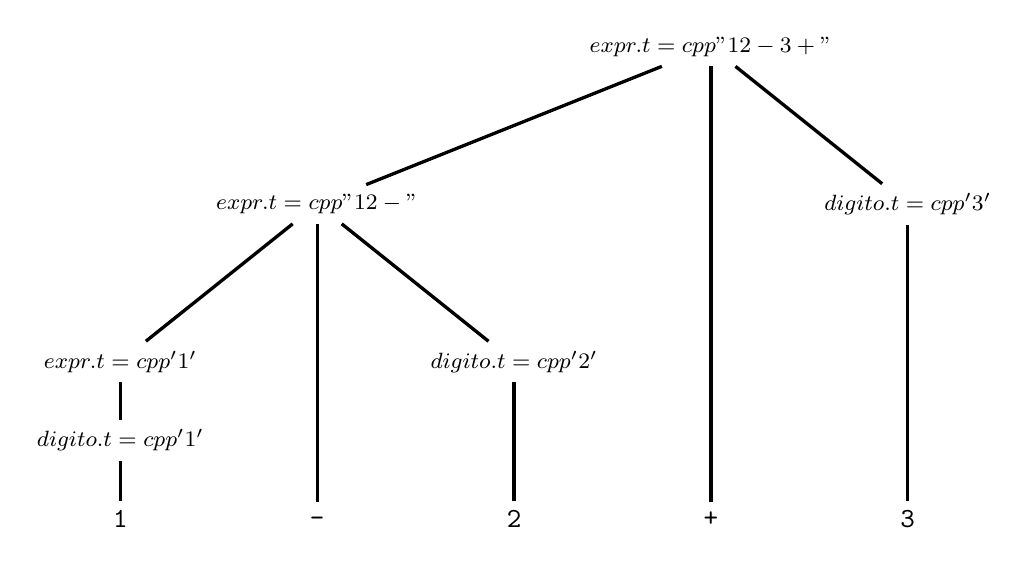
\begin{tikzpicture} 
            \node (A) at (0, 0) { \texttt{1} };
            \node (B) at (0, 1) { \footnotesize $digito.t = \code{cpp}{'1'}$ };
            \node (C) at (0, 2) { \footnotesize $expr.t = \code{cpp}{'1'}$ };
            \node (D) at (2.5, 0) { \texttt{-} };
            \node (E) at (2.5, 4) { \footnotesize $expr.t = \code{cpp}{"12-"}$ };
            \node (F) at (5, 0) { \texttt{2} };
            \node (G) at (5, 2) { \footnotesize $digito.t = \code{cpp}{'2'}$ };
            \node (H) at (7.5, 6) { \footnotesize $expr.t = \code{cpp}{"12-3+"}$ };
            \node (I) at (7.5, 0) { \texttt{+} };
            \node (J) at (10, 4) { \footnotesize $digito.t = \code{cpp}{'3'}$ };
            \node (K) at (10, 0) { \texttt{3} };

            \draw[very thick] (A) to (B);
            \draw[very thick] (C) to (B);
            \draw[very thick] (C) to (E);
            \draw[very thick] (E) to (D);
            \draw[very thick] (F) to (G);
            \draw[very thick] (E) to (G);
            \draw[very thick] (E) to (H);
            \draw[very thick] (I) to (H);
            \draw[very thick] (H) to (J);
            \draw[very thick] (K) to (J);
        \end{tikzpicture} 
    \end{figure}

\end{frame}

\begin{frame}[fragile]{Esquema de tradução}

    \begin{itemize}
        \item Um esquema de tradução é uma gramática livre de contexto na qual fragmentos de programas, denominados ações semânticas, são inseridos nos lados
            direitos das produções
       %\pause

        \item Num esquema de tradução, a ordem de avaliação das ações semânticas é explicitamente mostrada
       %\pause

        \item A posição na qual uma ação semântica deve ser executada é marcada no lado direito da produção, por meio de chaves
       %\pause

        \item Na árvore gramatical uma ação semântica é indicada por um filho extra, conectado por meio de uma linha pontilhada
       %\pause

        \item Nós rotulados por ações gramaticas não possui filhos
    \end{itemize}

\end{frame}

\begin{frame}[fragile]{Ações semânticas para a tradução de expressões para a notação posfixa}

\[
    \begin{array}{lcl}
        expr & \to & expr + digito\ \ \ \ \{ imprimir(\code{cpp}{'+'}) \} \\
        expr & \to & expr - digito\ \ \ \ \{ imprimir(\code{cpp}{'-'})\} \\
        expr & \to & digito \\
        digito & \to & 0 \ \ \ \ \{ imprimir(\code{cpp}{'0'}) \} \\
        digito & \to & 1 \ \ \ \ \{ imprimir(\code{cpp}{'1'}) \} \\
        & $\ldots$ \\
        digito & \to & 9 \ \ \ \ \{ imprimir(\code{cpp}{'9'}) \} \\
    \end{array}
\]

\end{frame}

\begin{frame}[fragile]{Árvore gramatical com ações semânticas que traduz a expressão \code{cpp}{1-2+3}}

    \begin{figure}
        \centering

        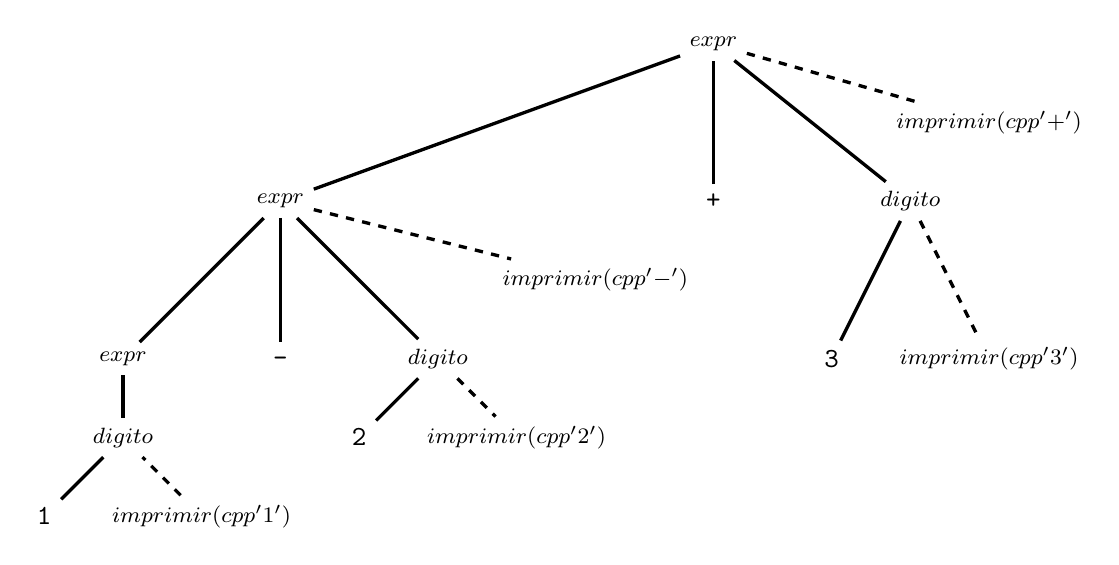
\begin{tikzpicture} 
            \node (A) at (-1, 0) { \texttt{1} };
            \node (A1) at (1, 0) { \footnotesize $imprimir(\code{cpp}{'1'})$ };
            \node (B) at (0, 1) { \footnotesize $digito$ };
            \node (C) at (0, 2) { \footnotesize $expr$ };
            \node (D) at (2, 2) { \texttt{-} };
            \node (E) at (2, 4) { \footnotesize $expr$ };
            \node (E1) at (6, 3) { \footnotesize $imprimir(\code{cpp}{'-'})$ };
            \node (F) at (3, 1) { \texttt{2} };
            \node (F1) at (5, 1) { \footnotesize $imprimir(\code{cpp}{'2'})$ };
            \node (G) at (4, 2) { \footnotesize $digito$ };
            \node (H) at (7.5, 6) { \footnotesize $expr$ };
            \node (I) at (7.5, 4) { \texttt{+} };
            \node (J) at (10, 4) { \footnotesize $digito$ };
            \node (K) at (9, 2) { \texttt{3} };
            \node (K1) at (11, 2) { \footnotesize $imprimir(\code{cpp}{'3'})$ };
            \node (L) at (11, 5) { \footnotesize $imprimir(\code{cpp}{'+'})$ };

            \draw[very thick] (A) to (B);
            \draw[very thick,dashed] (A1) to (B);
            \draw[very thick] (C) to (B);
            \draw[very thick] (C) to (E);
            \draw[very thick] (E) to (D);
            \draw[very thick,dashed] (E) to (E1);
            \draw[very thick] (F) to (G);
            \draw[very thick,dashed] (G) to (F1);
            \draw[very thick] (E) to (G);
            \draw[very thick] (E) to (H);
            \draw[very thick] (I) to (H);
            \draw[very thick] (H) to (J);
            \draw[very thick] (K) to (J);
            \draw[very thick,dashed] (J) to (K1);
            \draw[very thick,dashed] (H) to (L);
        \end{tikzpicture} 
    \end{figure}

\end{frame}


